\chapter{Simulazioni}

\section{Simulazione SIL}

\subsection{PID}
\subsubsection{STEP}
\todo[inline]{Tabella dei waypoints}
\begin{figure}
	\centering
	\begin{subfigure}{0.45\textwidth}
		\centering
		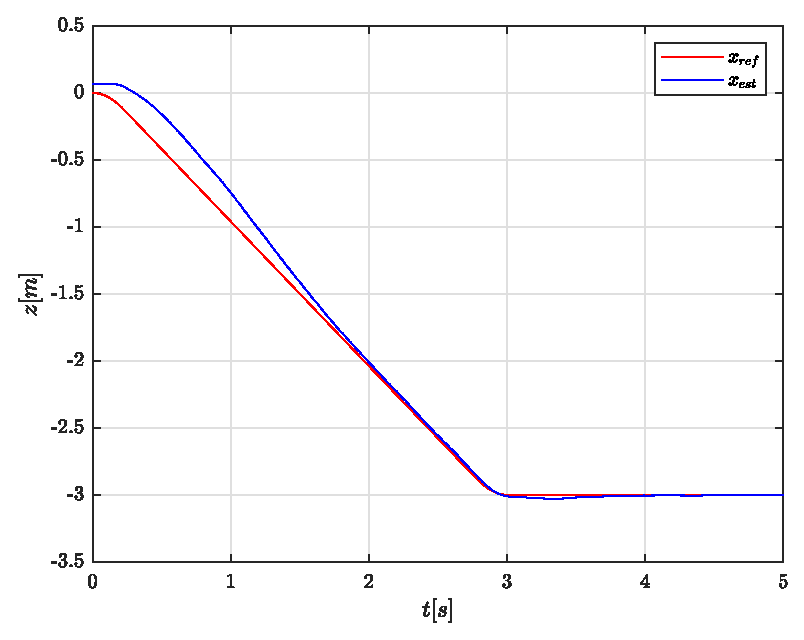
\includegraphics[width=1\textwidth]{Simulazioni/Figure/PID/STEP/AltitudeControlPos}
		\caption{Controllo posizione}
	\end{subfigure}
	\hfill
	\begin{subfigure}{0.45\textwidth}
		\centering
		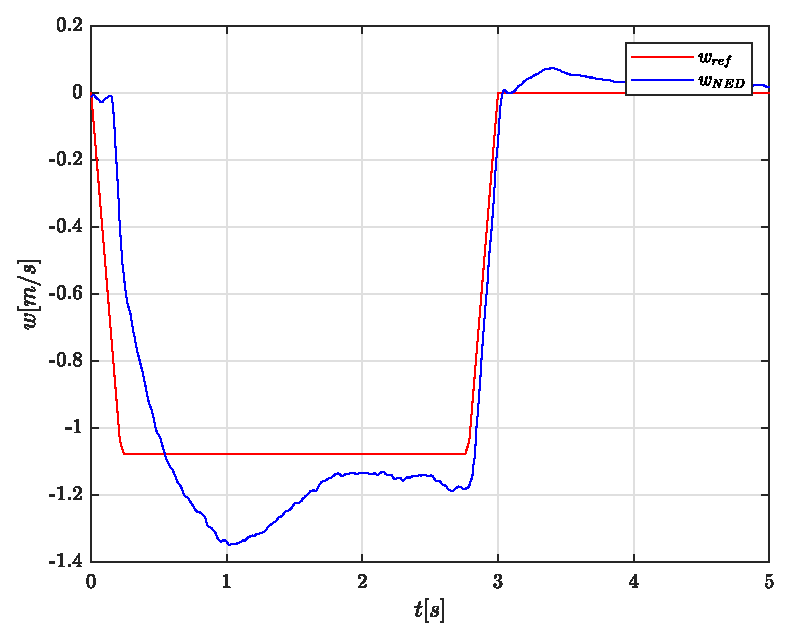
\includegraphics[width=1\textwidth]{Simulazioni/Figure/PID/STEP/AltitudeControlVel}
		\caption{Controllo velocità}
	\end{subfigure}
	\caption{Risposta del controllore PID di quota al segnale STEP}
\end{figure}

\begin{figure}
	\centering
	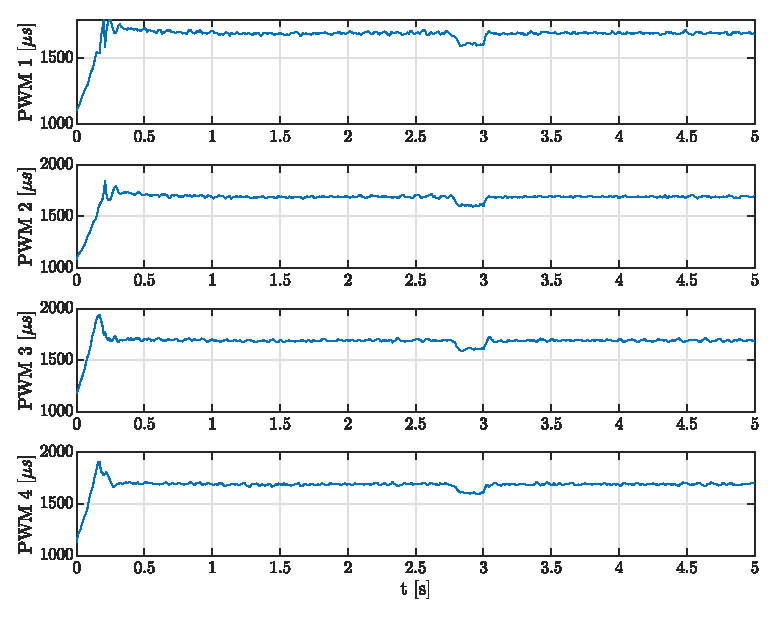
\includegraphics[width=0.5\textwidth]{Simulazioni/Figure/PID/STEP/PWM}
	\caption{Segnali PWM del controllore PID al segnale STEP}
\end{figure}
\clearpage
\subsubsection{SQUARE}
\begin{figure}
	\centering
	\begin{subfigure}{0.45\textwidth}
		\centering
		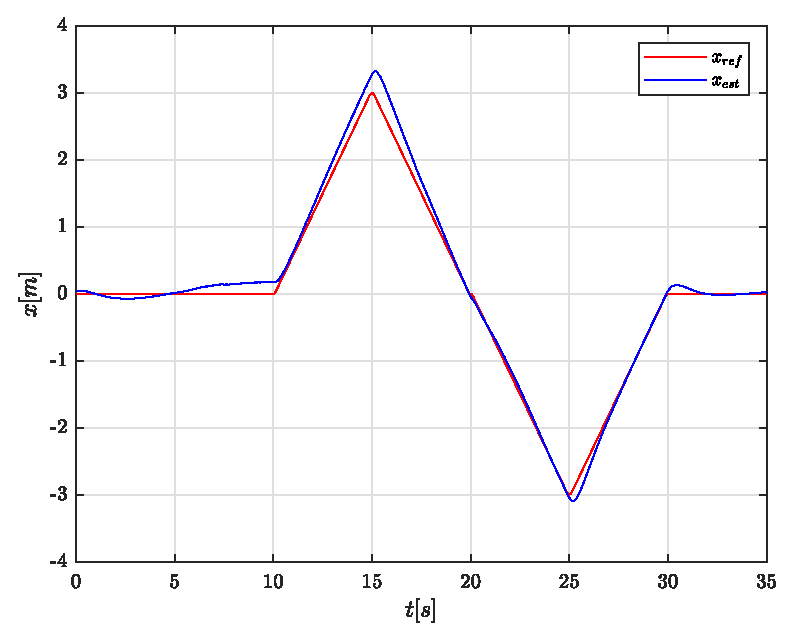
\includegraphics[width=1\textwidth]{Simulazioni/Figure/PID/SQUARE/PositionControlXPos}
		\caption{Controllo posizione lungo x}
	\end{subfigure}
	\hfill
	\begin{subfigure}{0.45\textwidth}
		\centering
		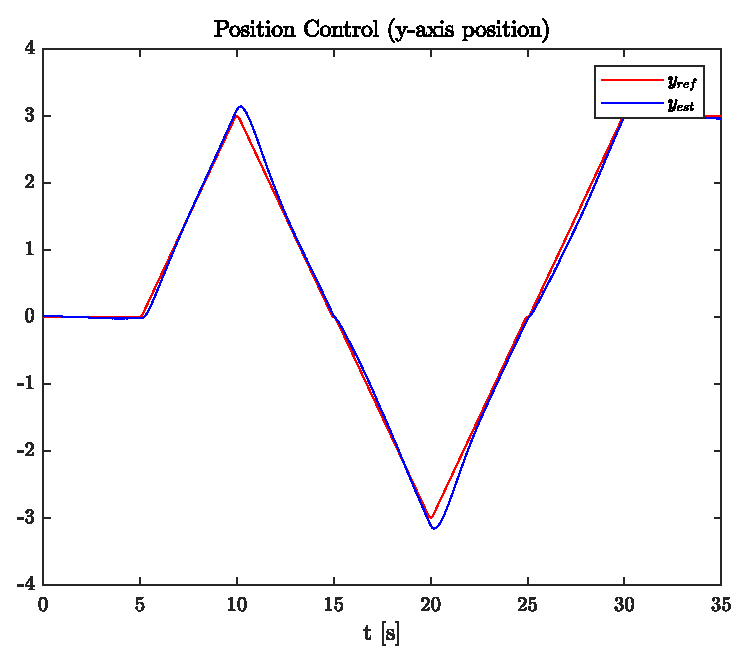
\includegraphics[width=1\textwidth]{Simulazioni/Figure/PID/SQUARE/PositionControlYPos}
		\caption{Controllo posizione lungo y}
	\end{subfigure}
	\\
	\begin{subfigure}{0.45\textwidth}
		\centering
		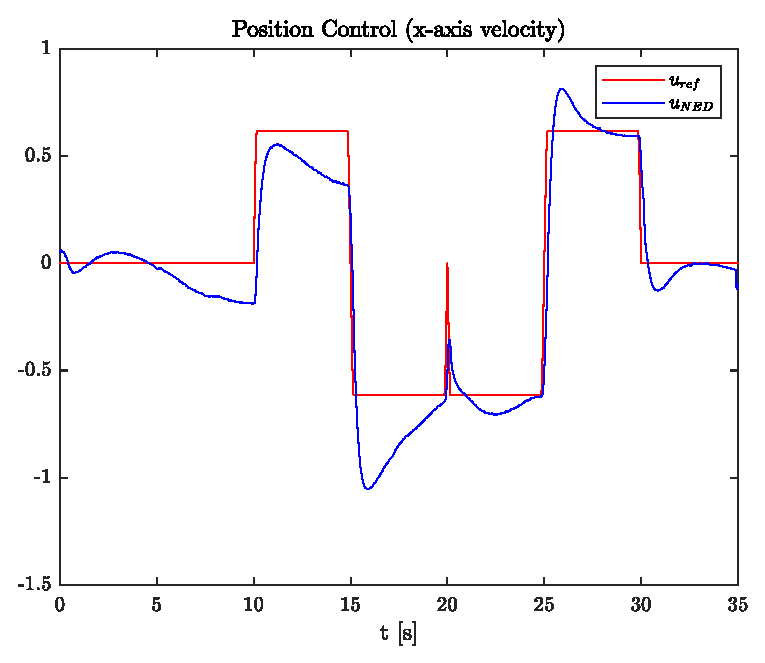
\includegraphics[width=1\textwidth]{Simulazioni/Figure/PID/SQUARE/PositionControlXVel}
		\caption{Controllo velocità lungo x}
	\end{subfigure}
	\hfill
	\begin{subfigure}{0.45\textwidth}
		\centering
		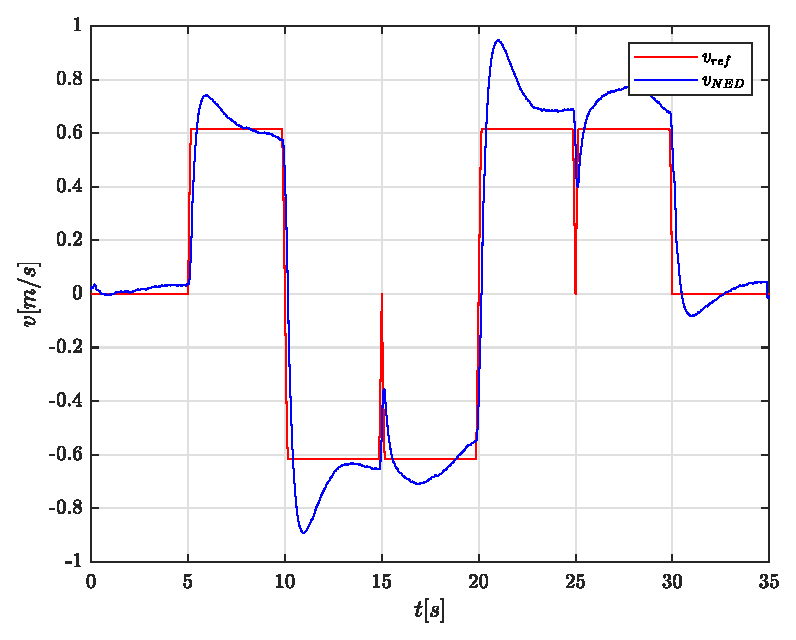
\includegraphics[width=1\textwidth]{Simulazioni/Figure/PID/SQUARE/PositionControlYVel}
		\caption{Controllo velocità lungo y}
	\end{subfigure}
	\caption{Risposta in posizione con controllore interno PID al comando SQUARE}
\end{figure}

\begin{figure}
	\centering
	\begin{subfigure}{0.45\textwidth}
		\centering
		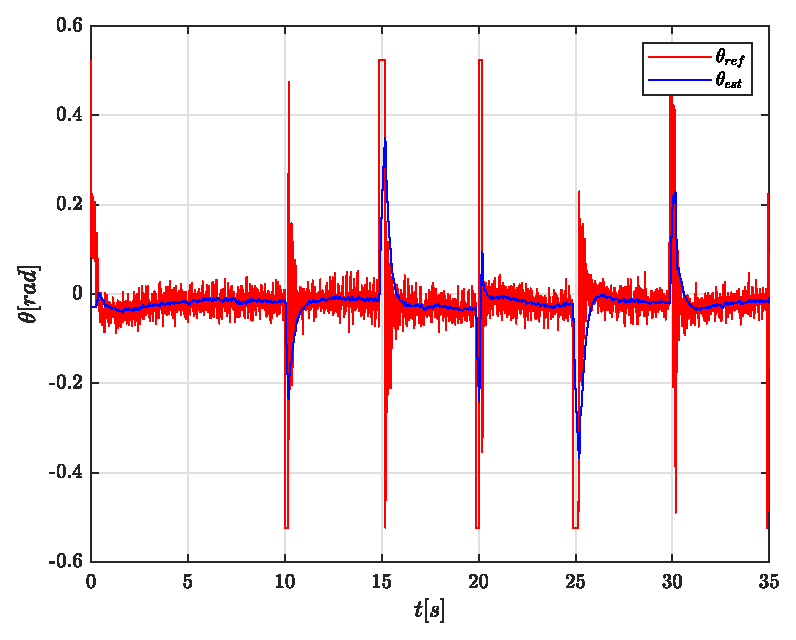
\includegraphics[width=1\textwidth]{Simulazioni/Figure/PID/SQUARE/AttitudeControlPitch}
		\caption{Controllo beccheggio}
	\end{subfigure}
	\hfill
	\begin{subfigure}{0.45\textwidth}
		\centering
		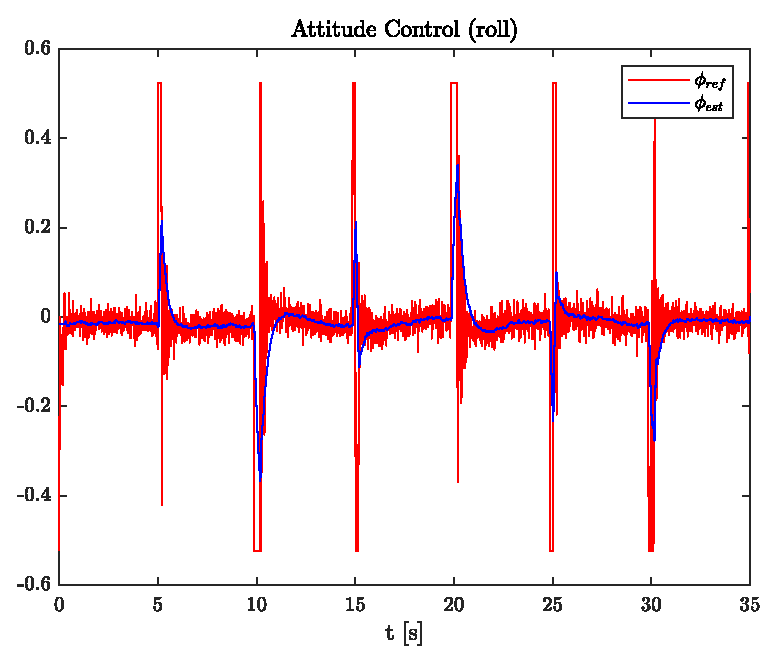
\includegraphics[width=1\textwidth]{Simulazioni/Figure/PID/SQUARE/AttitudeControlRoll}
		\caption{Controllo rollio}
	\end{subfigure}
	\hfill
	\begin{subfigure}{0.45\textwidth}
		\centering
		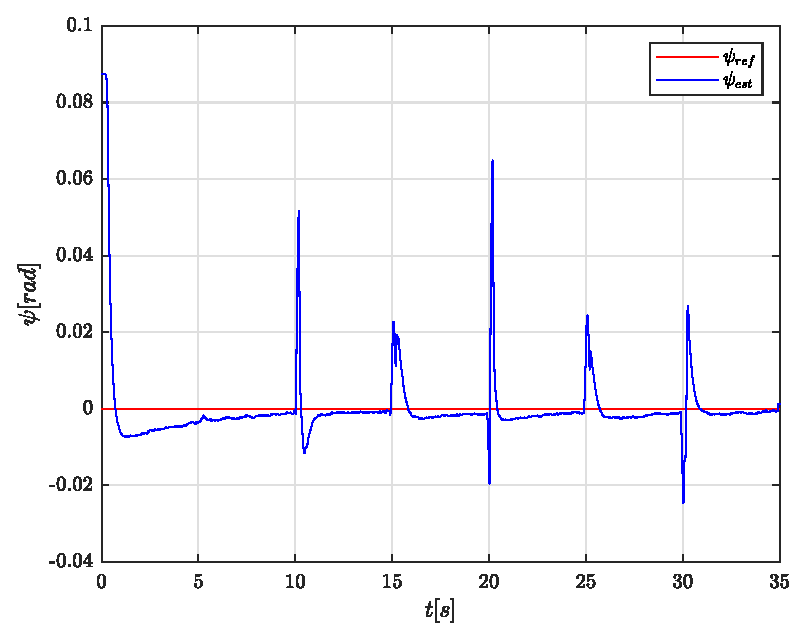
\includegraphics[width=1\textwidth]{Simulazioni/Figure/PID/SQUARE/AttitudeControlYaw}
		\caption{Controllo imbardata}
	\end{subfigure}
	\caption{Risposta dell' assetto con controllore interno PID al comando SQUARE}
\end{figure}


\begin{figure}
	\centering
	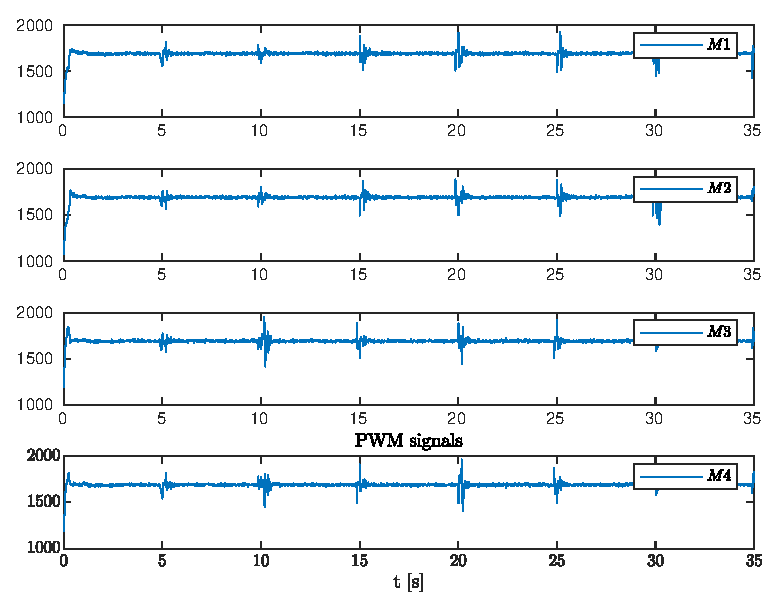
\includegraphics[width=0.5\textwidth]{Simulazioni/Figure/PID/SQUARE/PWM}
	\caption{Segnali PWM del controllore PID al segnale SQUARE}
\end{figure}
\begin{figure}
	\centering
	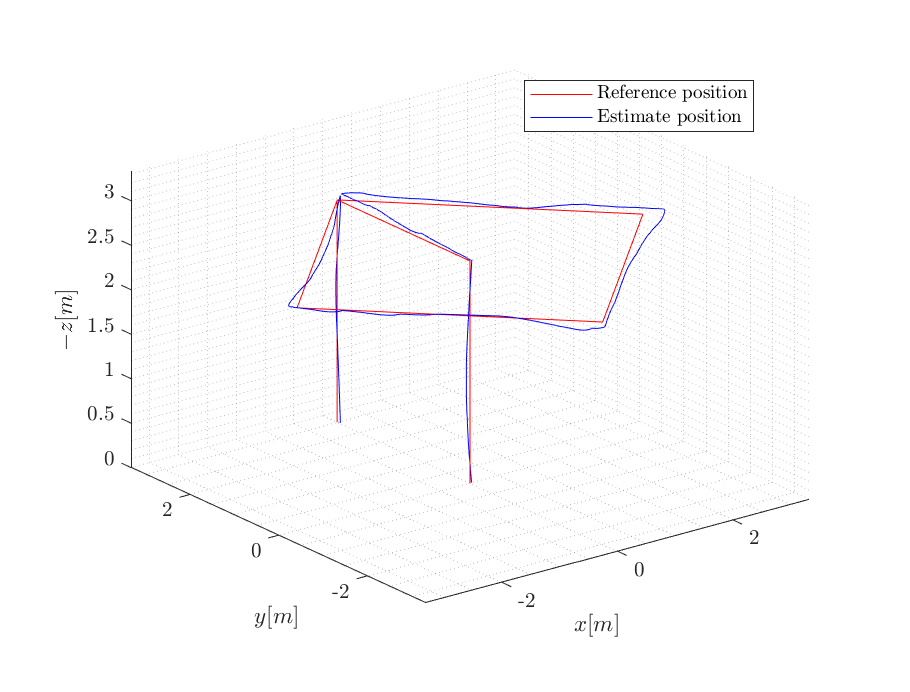
\includegraphics[width=1\textwidth]{Simulazioni/Figure/PID/SQUARE/Trajectory}
	\caption{Traiettoria percorsa con controllore PID al segnale SQUARE}
\end{figure}

\clearpage

\subsubsection{BUTTERFLY}
\begin{figure}
	\centering
	\begin{subfigure}{0.45\textwidth}
		\centering
		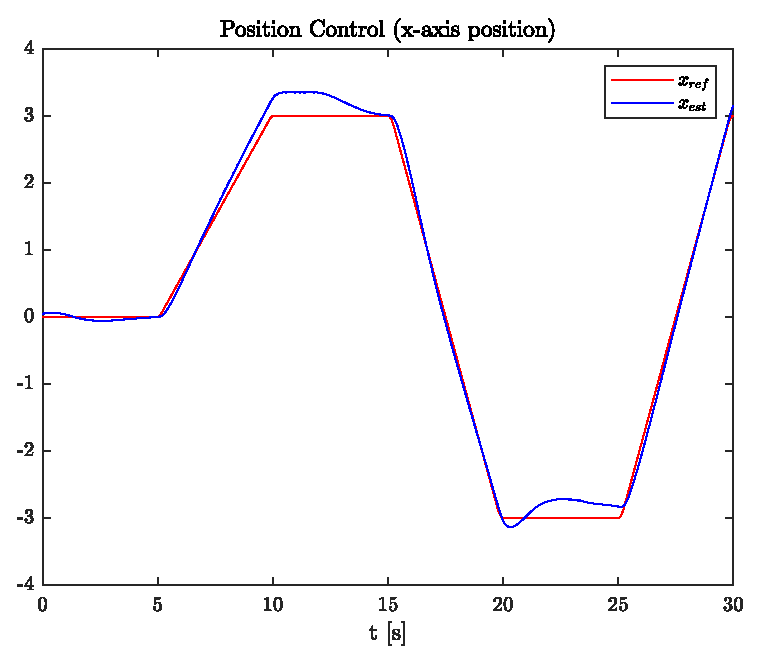
\includegraphics[width=1\textwidth]{Simulazioni/Figure/PID/BUTTERFLY/PositionControlXPos}
		\caption{Controllo posizione lungo x}
	\end{subfigure}
	\hfill
	\begin{subfigure}{0.45\textwidth}
		\centering
		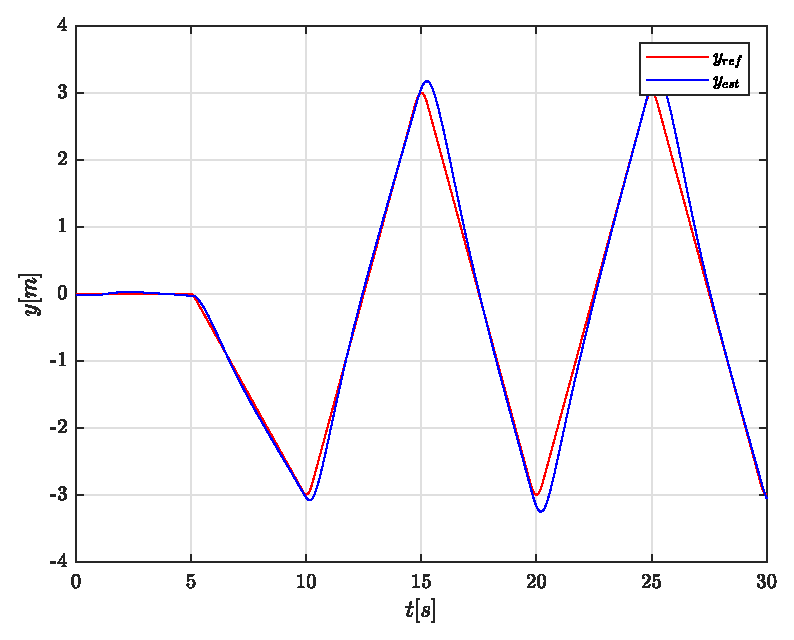
\includegraphics[width=1\textwidth]{Simulazioni/Figure/PID/BUTTERFLY/PositionControlYPos}
		\caption{Controllo posizione lungo y}
	\end{subfigure}
	\\
	\begin{subfigure}{0.45\textwidth}
		\centering
		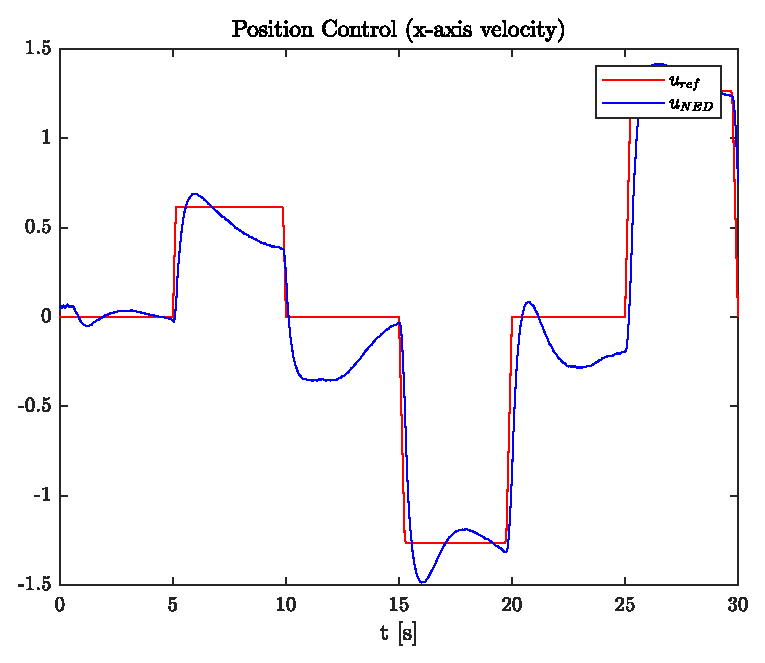
\includegraphics[width=1\textwidth]{Simulazioni/Figure/PID/BUTTERFLY/PositionControlXVel}
		\caption{Controllo velocità lungo x}
	\end{subfigure}
	\hfill
	\begin{subfigure}{0.45\textwidth}
		\centering
		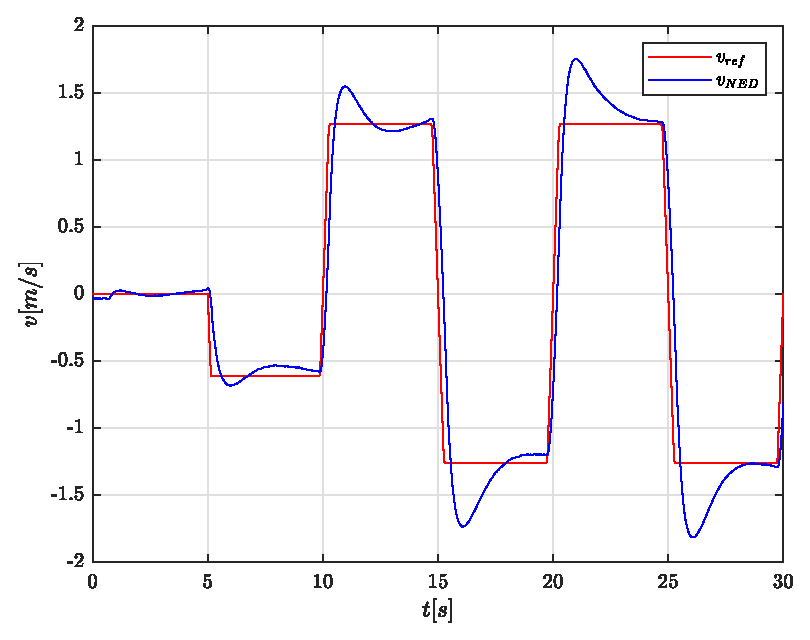
\includegraphics[width=1\textwidth]{Simulazioni/Figure/PID/BUTTERFLY/PositionControlYVel}
		\caption{Controllo velocità lungo y}
	\end{subfigure}
	\caption{Risposta in posizione con controllore interno PID al comando BUTTERFLY}
\end{figure}

\begin{figure}
	\centering
	\begin{subfigure}{0.45\textwidth}
		\centering
		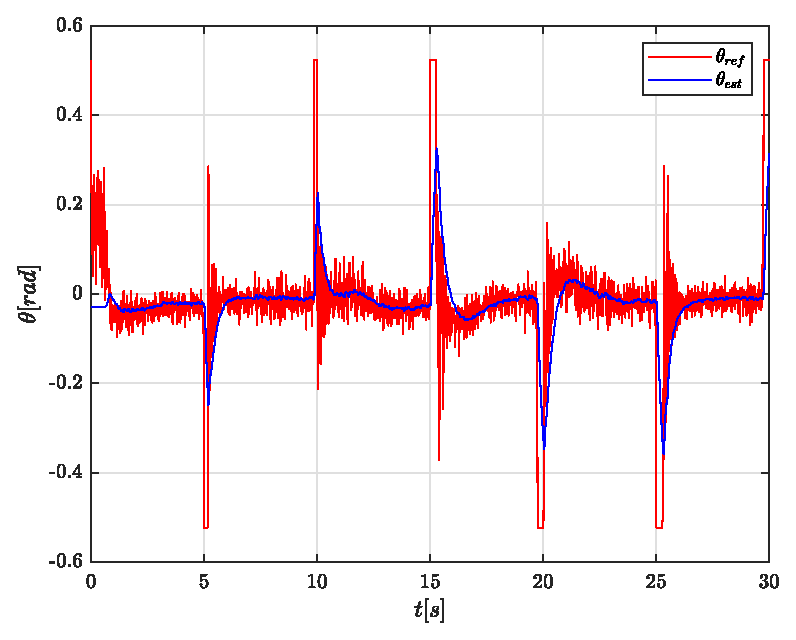
\includegraphics[width=1\textwidth]{Simulazioni/Figure/PID/BUTTERFLY/AttitudeControlPitch}
		\caption{Controllo beccheggio}
	\end{subfigure}
	\hfill
	\begin{subfigure}{0.45\textwidth}
		\centering
		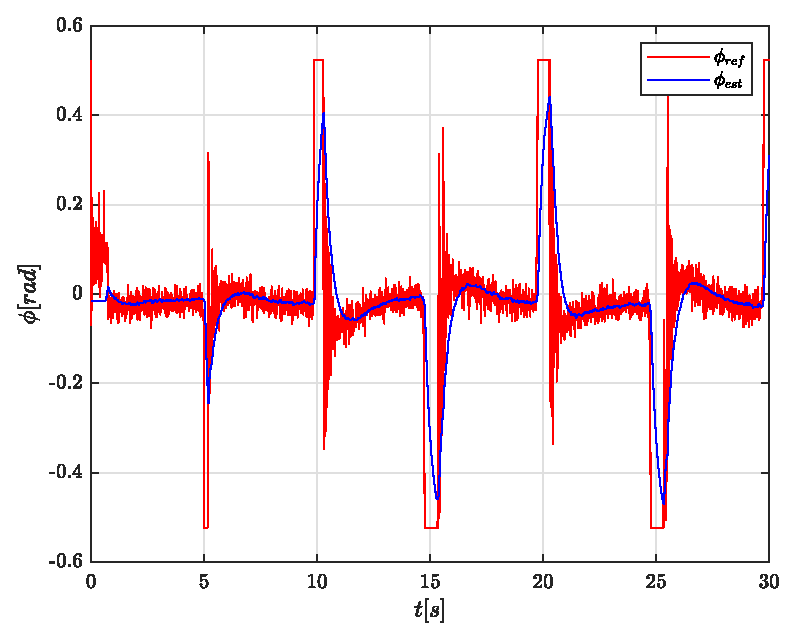
\includegraphics[width=1\textwidth]{Simulazioni/Figure/PID/BUTTERFLY/AttitudeControlRoll}
		\caption{Controllo rollio}
	\end{subfigure}
	\hfill
	\begin{subfigure}{0.45\textwidth}
		\centering
		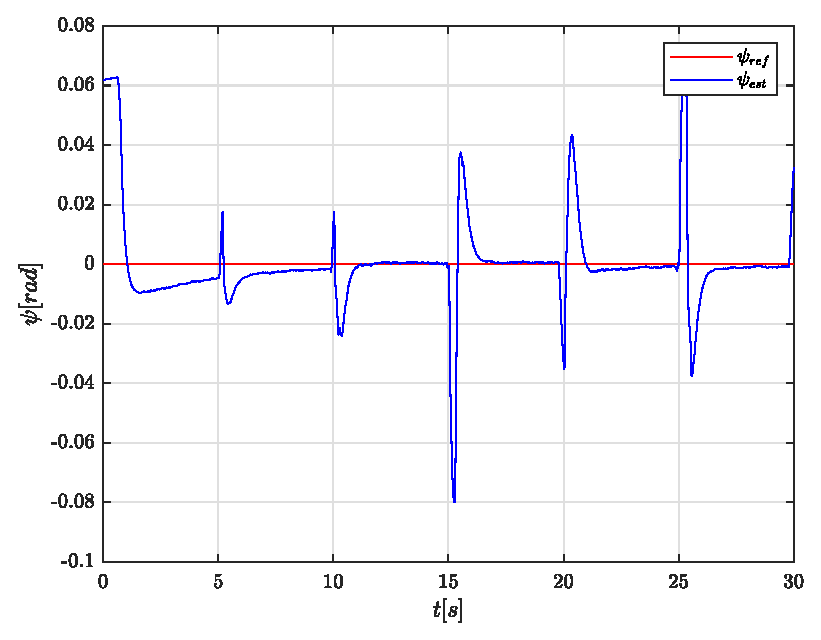
\includegraphics[width=1\textwidth]{Simulazioni/Figure/PID/BUTTERFLY/AttitudeControlYaw}
		\caption{Controllo imbardata}
	\end{subfigure}
	\caption{Risposta dell' assetto con controllore interno PID al comando BUTTERFLY}
\end{figure}


\begin{figure}
	\centering
	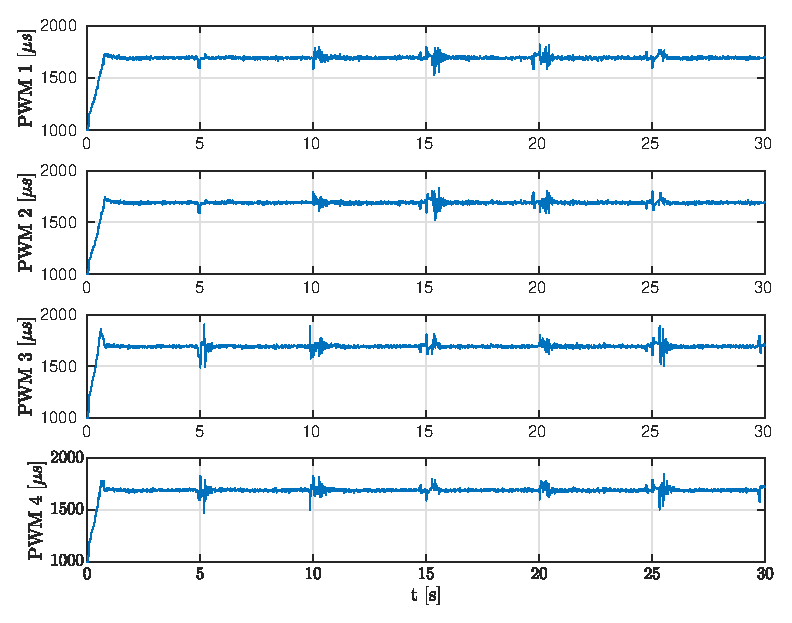
\includegraphics[width=0.5\textwidth]{Simulazioni/Figure/PID/BUTTERFLY/PWM}
	\caption{Segnali PWM del controllore PID al segnale BUTTERFLY}
\end{figure}
\begin{figure}
	\centering
	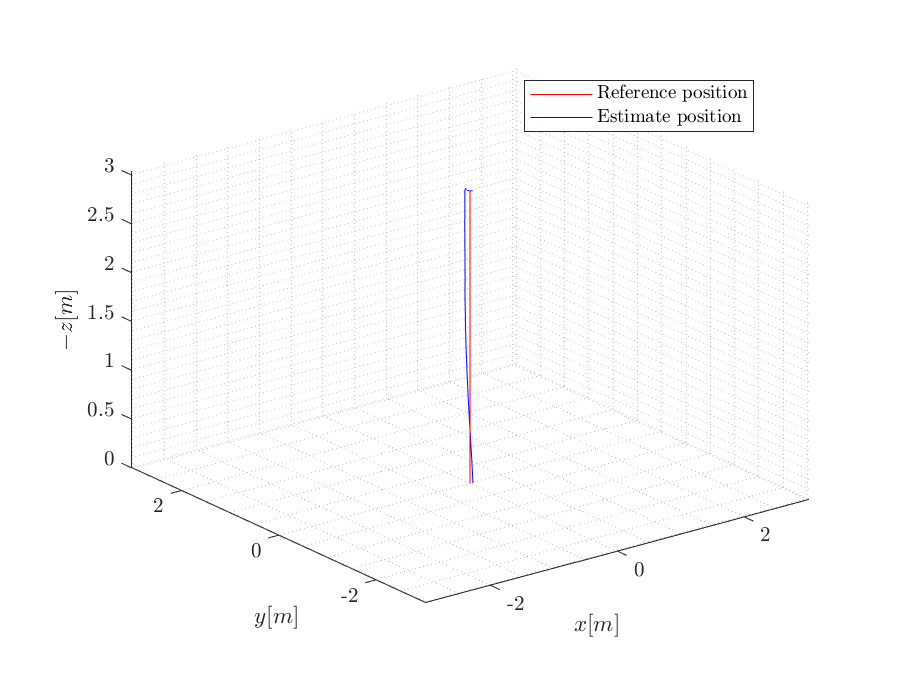
\includegraphics[width=1\textwidth]{Simulazioni/Figure/PID/BUTTERFLY/Trajectory}
	\caption{Traiettoria percorsa con controllore PID al segnale SQUARE}
\end{figure}

\clearpage
\subsubsection{SNAKE}
\begin{figure}
	\centering
	\begin{subfigure}{0.45\textwidth}
		\centering
		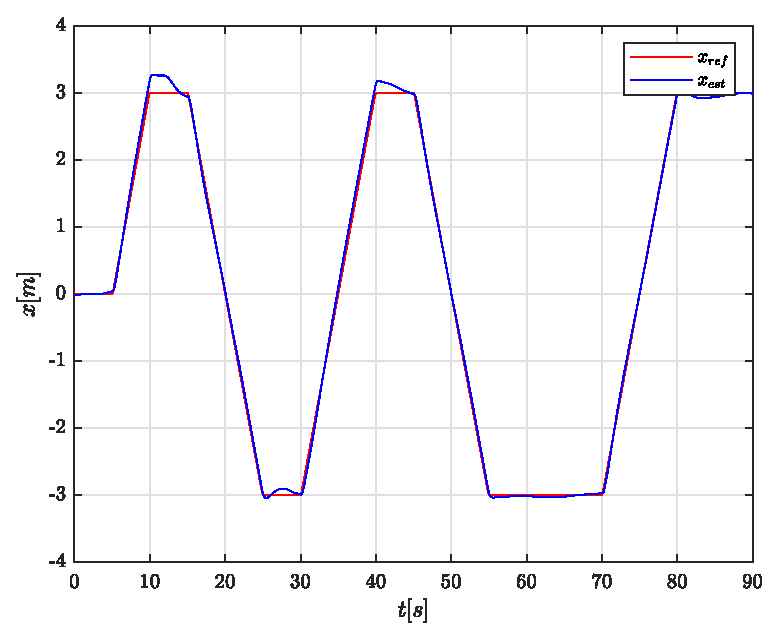
\includegraphics[width=1\textwidth]{Simulazioni/Figure/PID/SNAKE/PositionControlXPos}
		\caption{Controllo posizione lungo x}
	\end{subfigure}
	\hfill
	\begin{subfigure}{0.45\textwidth}
		\centering
		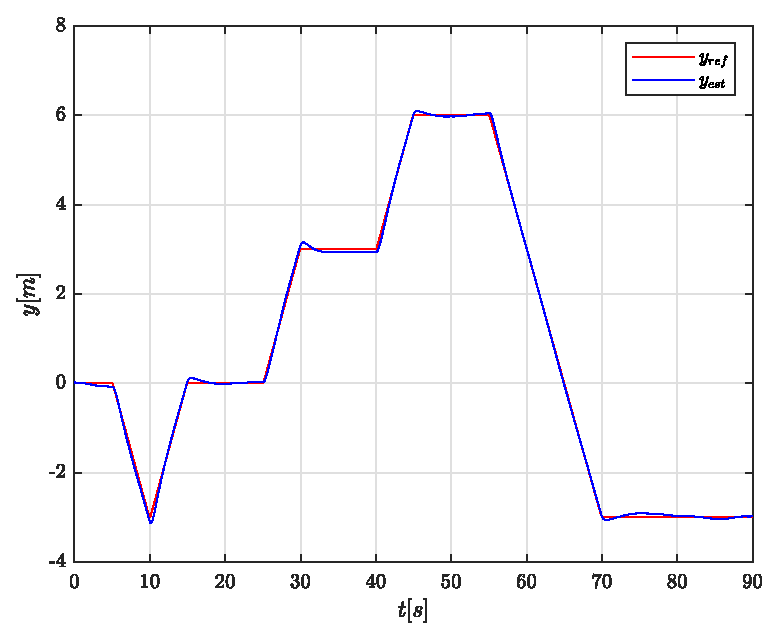
\includegraphics[width=1\textwidth]{Simulazioni/Figure/PID/SNAKE/PositionControlYPos}
		\caption{Controllo posizione lungo y}
	\end{subfigure}
	\\
	\begin{subfigure}{0.45\textwidth}
		\centering
		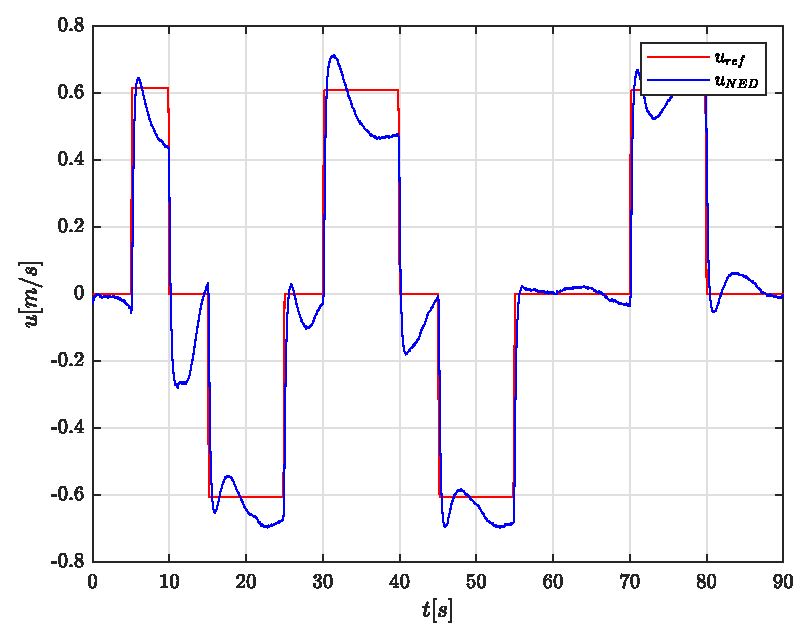
\includegraphics[width=1\textwidth]{Simulazioni/Figure/PID/SNAKE/PositionControlXVel}
		\caption{Controllo velocità lungo x}
	\end{subfigure}
	\hfill
	\begin{subfigure}{0.45\textwidth}
		\centering
		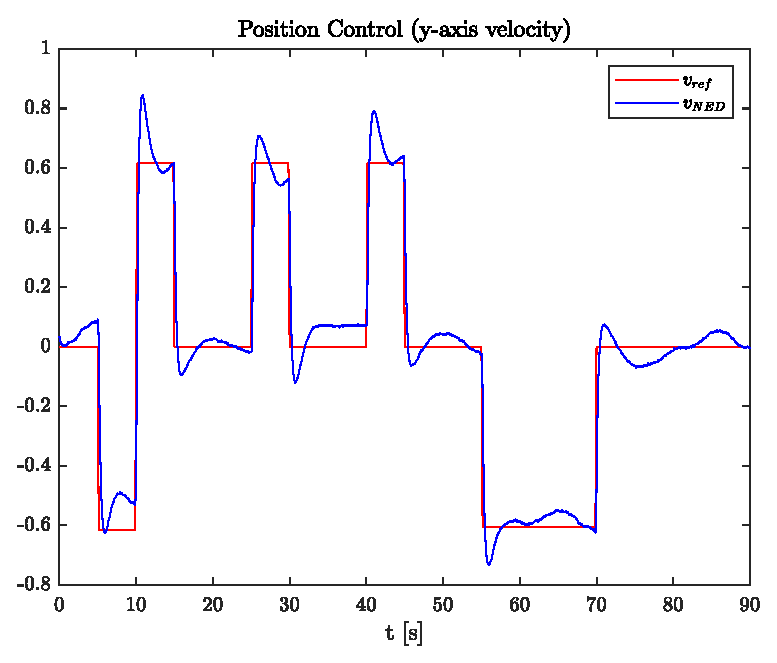
\includegraphics[width=1\textwidth]{Simulazioni/Figure/PID/SNAKE/PositionControlYVel}
		\caption{Controllo velocità lungo y}
	\end{subfigure}
	\caption{Risposta in posizione con controllore interno PID al comando SNAKE}
\end{figure}

\begin{figure}
	\centering
	\begin{subfigure}{0.45\textwidth}
		\centering
		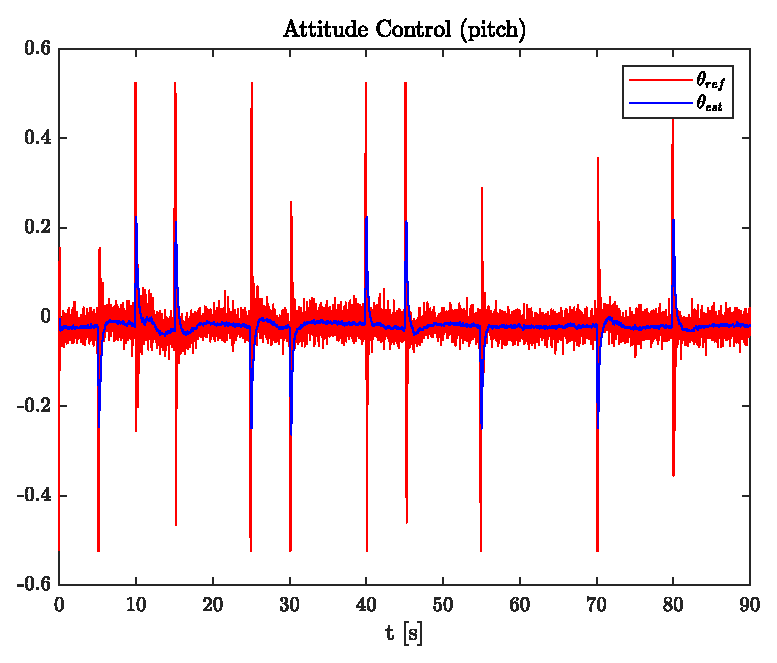
\includegraphics[width=1\textwidth]{Simulazioni/Figure/PID/SNAKE/AttitudeControlPitch}
		\caption{Controllo beccheggio}
	\end{subfigure}
	\hfill
	\begin{subfigure}{0.45\textwidth}
		\centering
		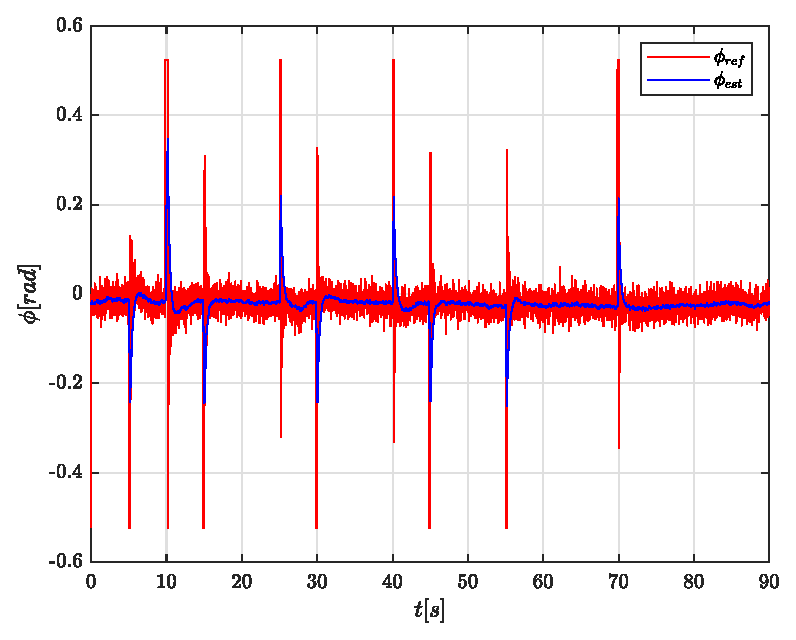
\includegraphics[width=1\textwidth]{Simulazioni/Figure/PID/SNAKE/AttitudeControlRoll}
		\caption{Controllo rollio}
	\end{subfigure}
	\hfill
	\begin{subfigure}{0.45\textwidth}
		\centering
		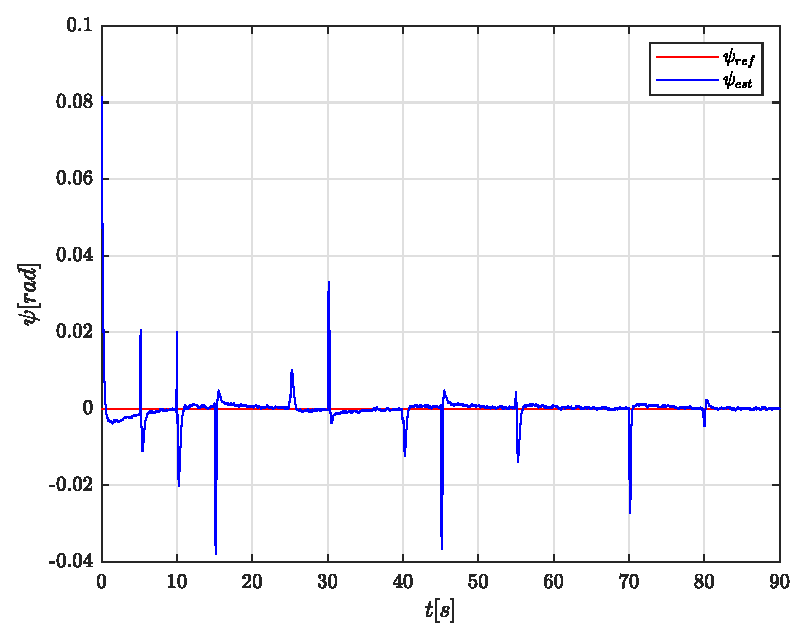
\includegraphics[width=1\textwidth]{Simulazioni/Figure/PID/SNAKE/AttitudeControlYaw}
		\caption{Controllo imbardata}
	\end{subfigure}
	\caption{Risposta dell' assetto con controllore interno PID al comando SNAKE}
\end{figure}


\begin{figure}
	\centering
	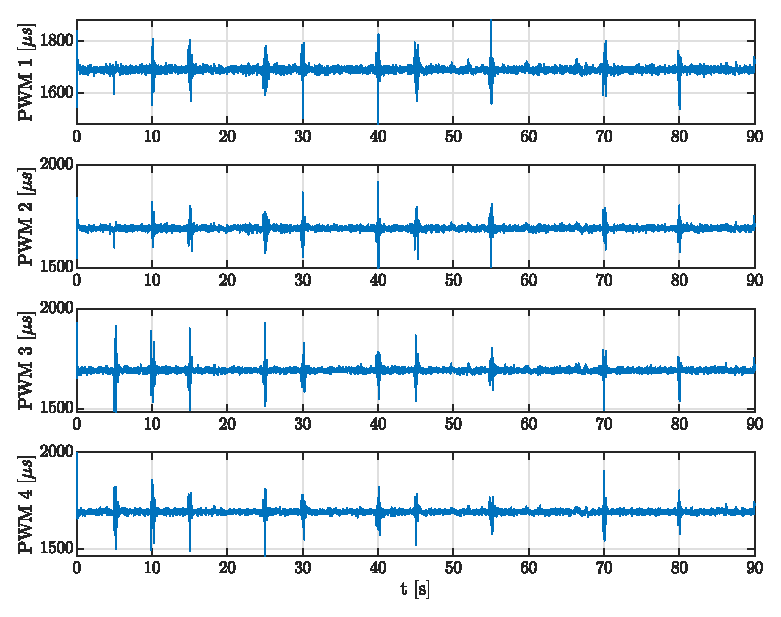
\includegraphics[width=0.5\textwidth]{Simulazioni/Figure/PID/SNAKE/PWM}
	\caption{Segnali PWM del controllore PID al segnale SNAKE}
\end{figure}
\begin{figure}
	\centering
	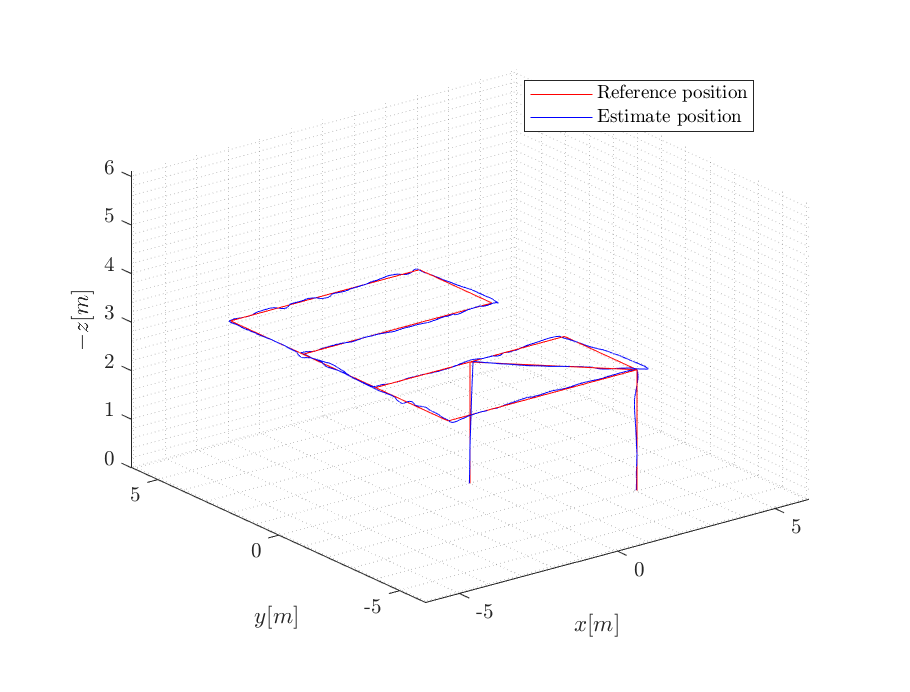
\includegraphics[width=1\textwidth]{Simulazioni/Figure/PID/SNAKE/Trajectory}
	\caption{Traiettoria percorsa con controllore PID al segnale SNAKE}
\end{figure}

\clearpage
\subsection{SMC}
\subsubsection{STEP}
\todo[inline]{Tabella dei waypoints}
\begin{figure}
	\centering
	\begin{subfigure}{0.45\textwidth}
		\centering
		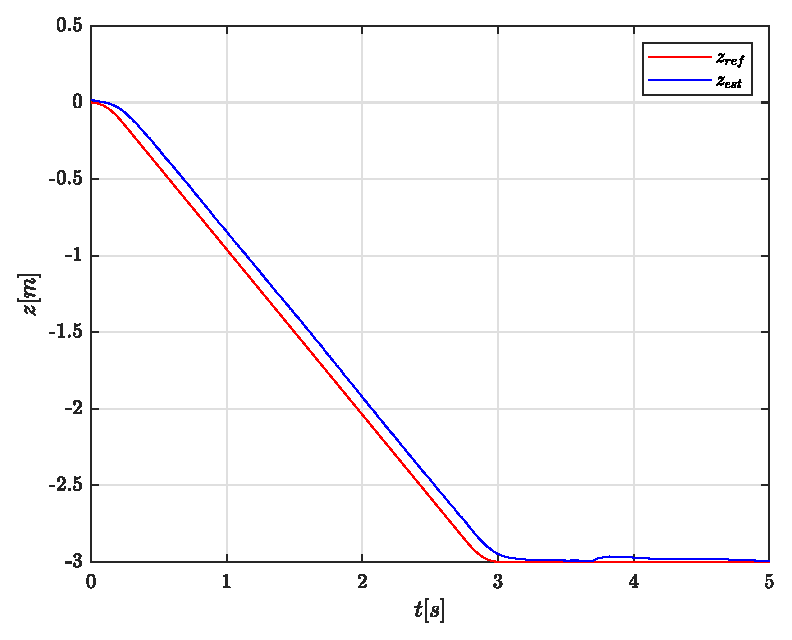
\includegraphics[width=1\textwidth]{Simulazioni/Figure/SMC/STEP/AltitudeControlPos}
		\caption{Controllo posizione}
	\end{subfigure}
	\hfill
	\begin{subfigure}{0.45\textwidth}
		\centering
		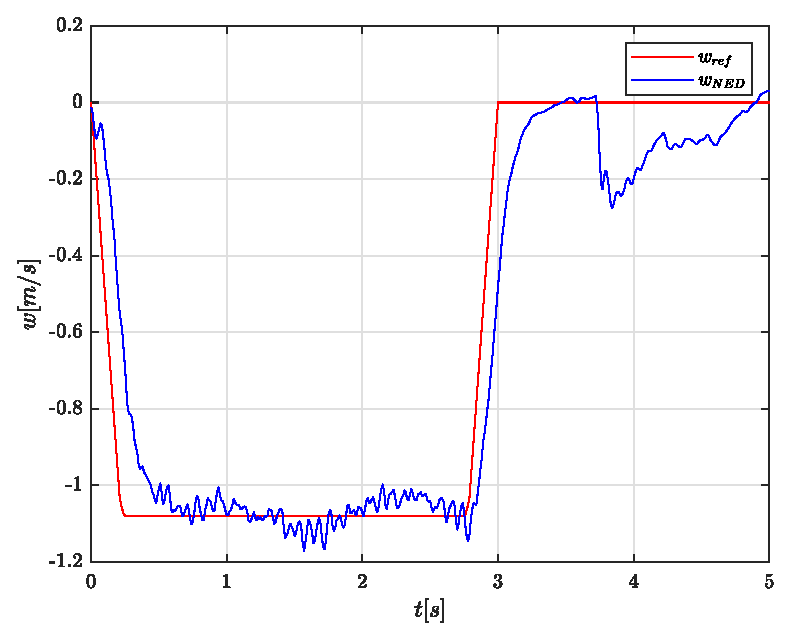
\includegraphics[width=1\textwidth]{Simulazioni/Figure/SMC/STEP/AltitudeControlVel}
		\caption{Controllo velocità}
	\end{subfigure}
	\caption{Risposta del controllore SMC di quota al segnale STEP}	
\end{figure}

\begin{figure}
	\centering
	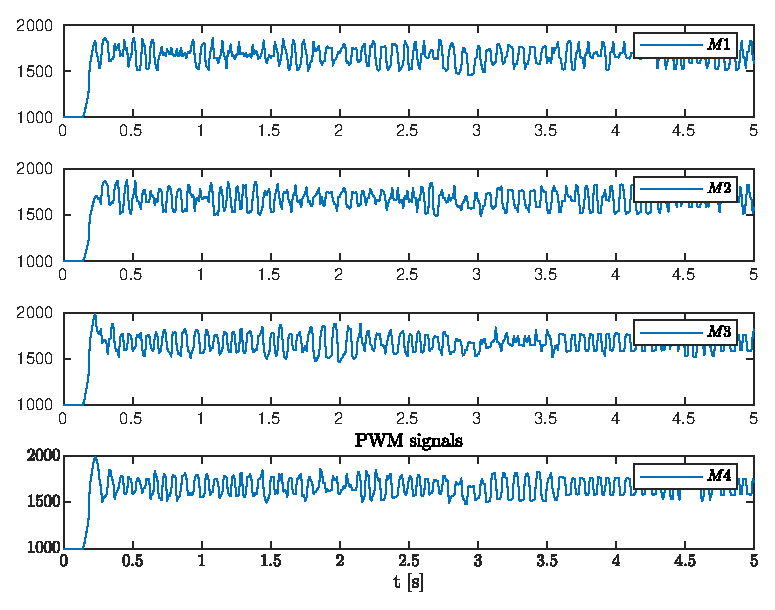
\includegraphics[width=0.5\textwidth]{Simulazioni/Figure/SMC/STEP/PWM}
	\caption{Segnali PWM generati del controllore SMC al segnale STEP}
\end{figure}
\clearpage

\subsubsection{SQUARE}
\begin{figure}
	\centering
	\begin{subfigure}{0.45\textwidth}
		\centering
		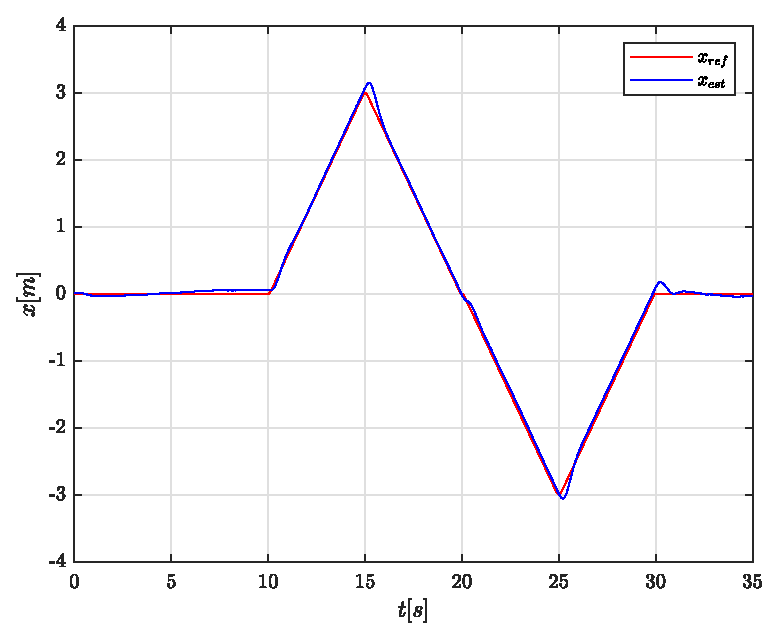
\includegraphics[width=1\textwidth]{Simulazioni/Figure/SMC/SQUARE/PositionControlXPos}
		\caption{Controllo posizione lungo x}
	\end{subfigure}
	\hfill
	\begin{subfigure}{0.45\textwidth}
		\centering
		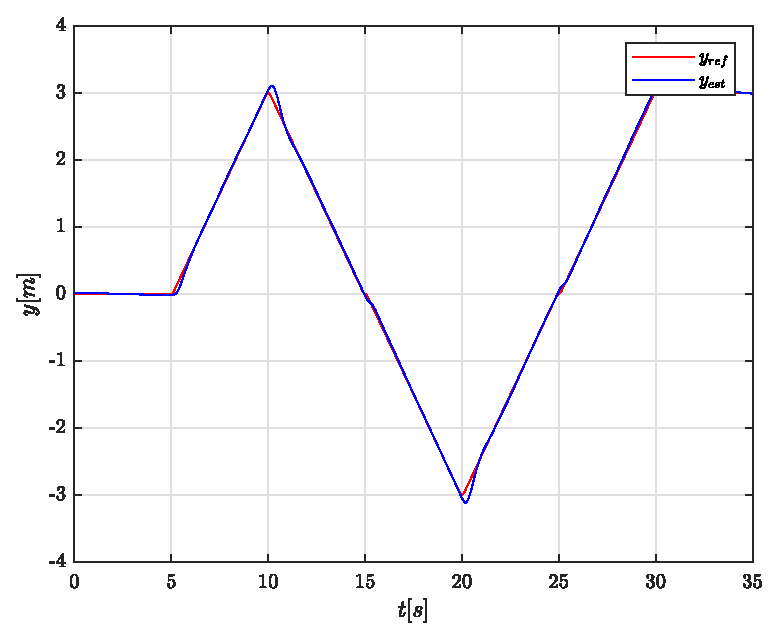
\includegraphics[width=1\textwidth]{Simulazioni/Figure/SMC/SQUARE/PositionControlYPos}
		\caption{Controllo posizione lungo y}
	\end{subfigure}
	\\
	\begin{subfigure}{0.45\textwidth}
		\centering
		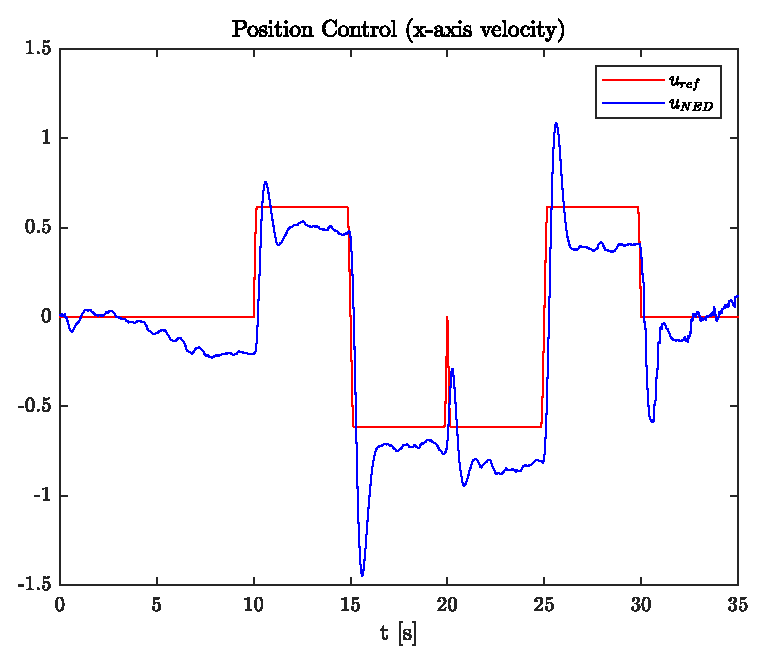
\includegraphics[width=1\textwidth]{Simulazioni/Figure/SMC/SQUARE/PositionControlXVel}
		\caption{Controllo velocità lungo x}
	\end{subfigure}
	\hfill
	\begin{subfigure}{0.45\textwidth}
		\centering
		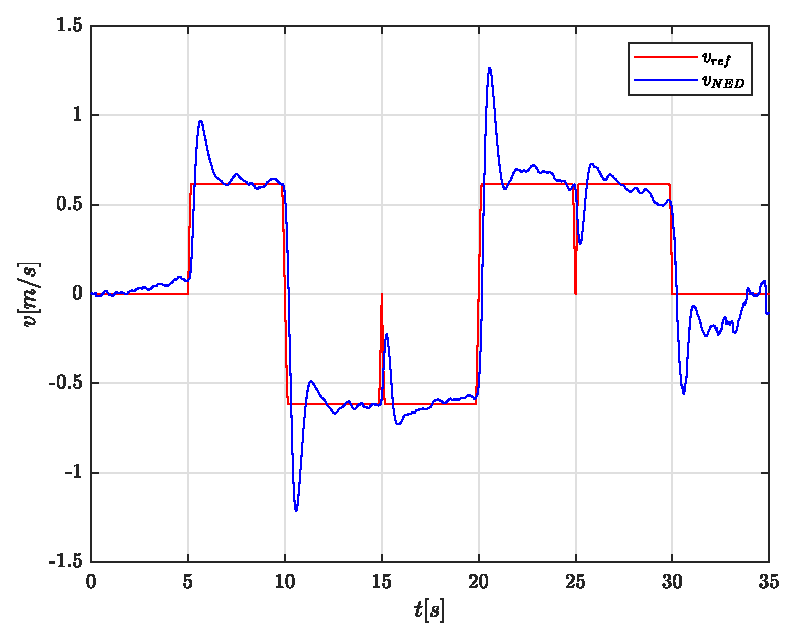
\includegraphics[width=1\textwidth]{Simulazioni/Figure/SMC/SQUARE/PositionControlYVel}
		\caption{Controllo velocità lungo y}
	\end{subfigure}
	\caption{Risposta del controllo posizione con controllore SMC al comando SQUARE}
\end{figure}

\begin{figure}
	\centering
	\begin{subfigure}{0.45\textwidth}
		\centering
		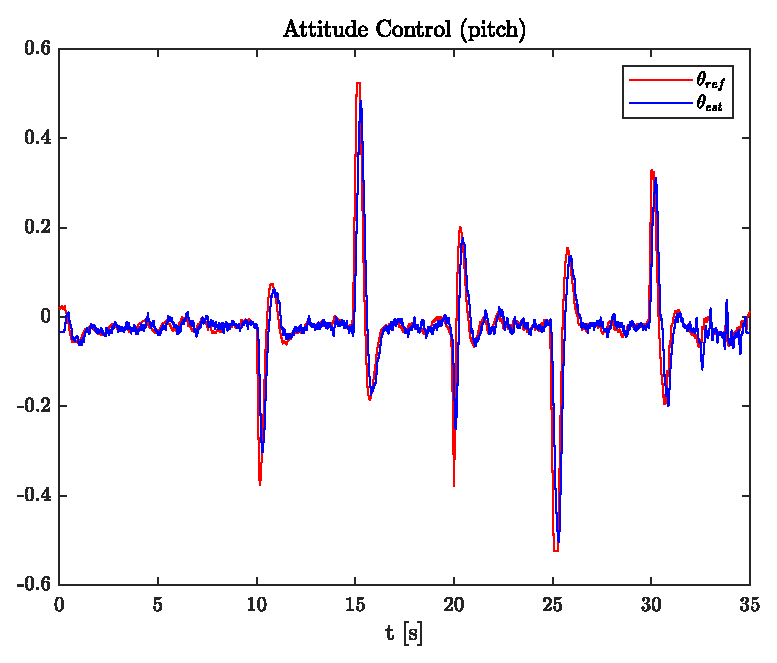
\includegraphics[width=1\textwidth]{Simulazioni/Figure/SMC/SQUARE/AttitudeControlPitch}
		\caption{Controllo beccheggio}
	\end{subfigure}
	\hfill
	\begin{subfigure}{0.45\textwidth}
		\centering
		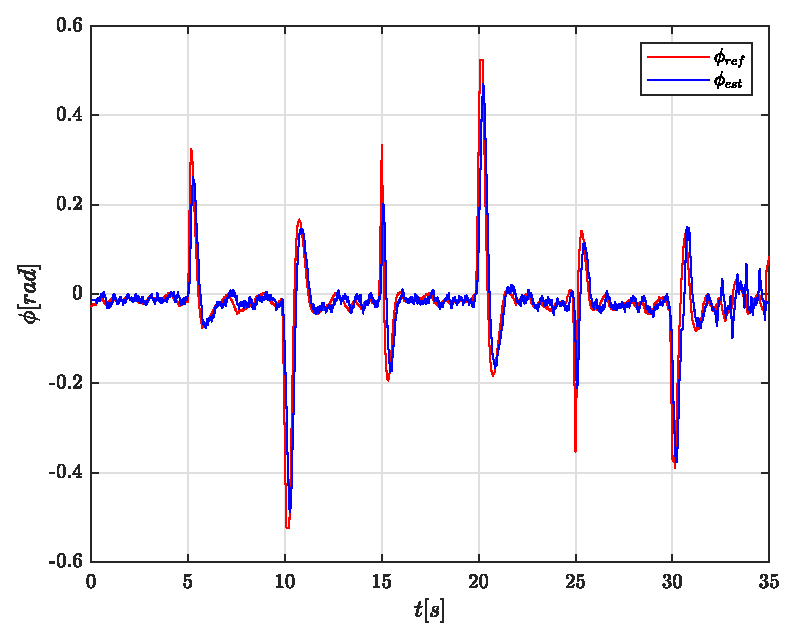
\includegraphics[width=1\textwidth]{Simulazioni/Figure/SMC/SQUARE/AttitudeControlRoll}
		\caption{Controllo rollio}
	\end{subfigure}
	\hfill
	\begin{subfigure}{0.45\textwidth}
		\centering
		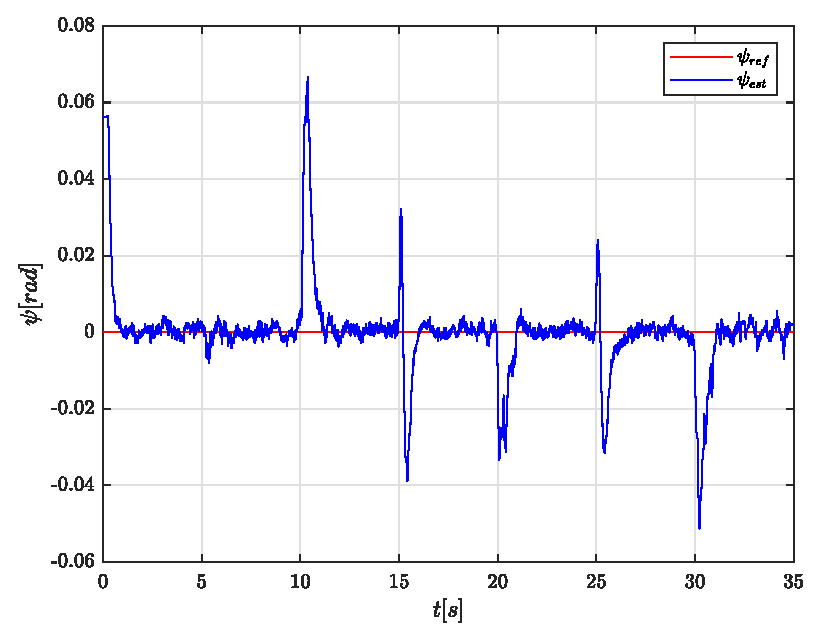
\includegraphics[width=1\textwidth]{Simulazioni/Figure/SMC/SQUARE/AttitudeControlYaw}
		\caption{Controllo imbardata}
	\end{subfigure}
	\caption{Risposta dell' assetto con controllore interno SMC al comando SQUARE}
\end{figure}


\begin{figure}
	\centering
	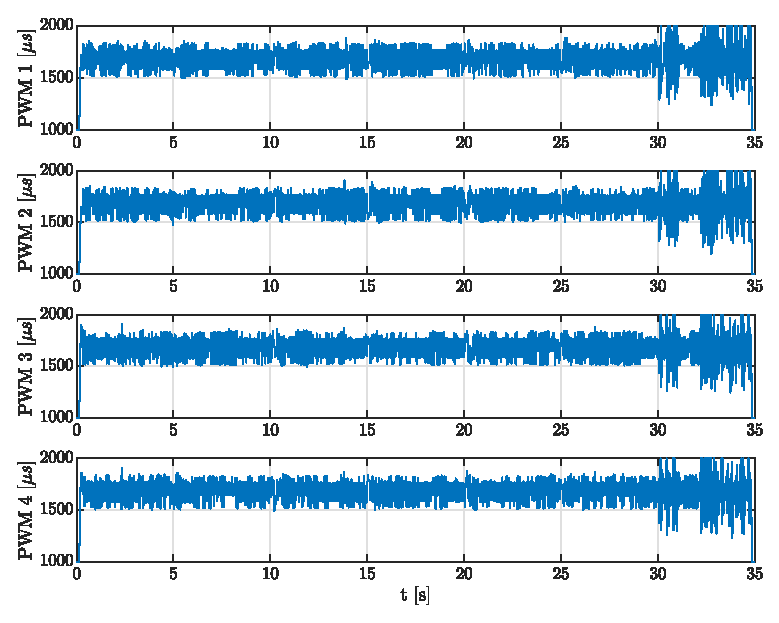
\includegraphics[width=0.5\textwidth]{Simulazioni/Figure/SMC/SQUARE/PWM}
	\caption{Segnali PWM del controllore SMC al segnale SQUARE}
\end{figure}
\begin{figure}
	\centering
	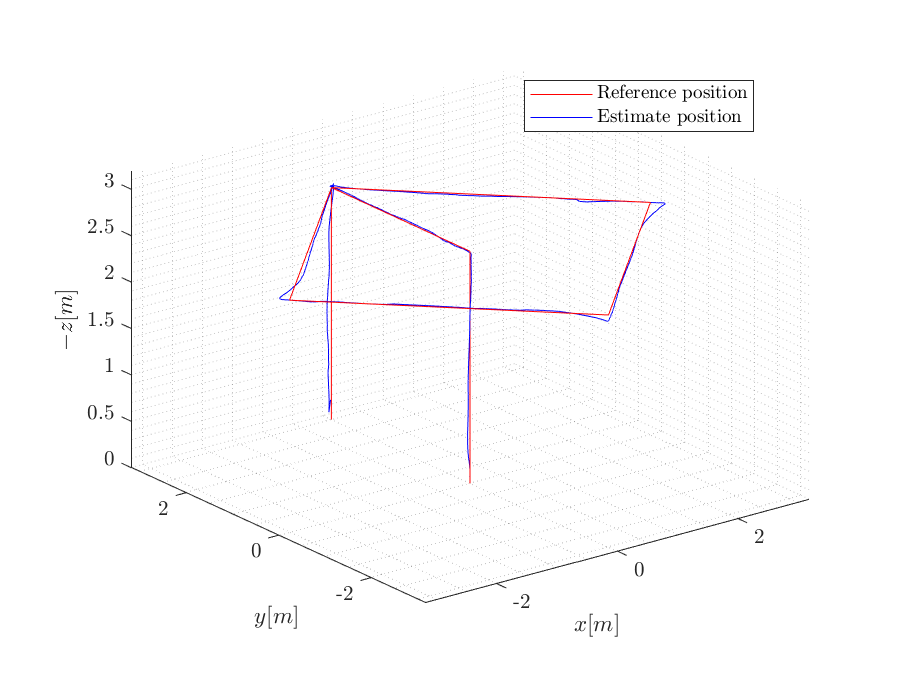
\includegraphics[width=1\textwidth]{Simulazioni/Figure/SMC/SQUARE/Trajectory}
	\caption{Traiettoria percorsa con controllore SMC al segnale SQUARE}
\end{figure}

\clearpage
\subsubsection{BUTTERFLY}

\begin{figure}
	\centering
	\begin{subfigure}{0.45\textwidth}
		\centering
		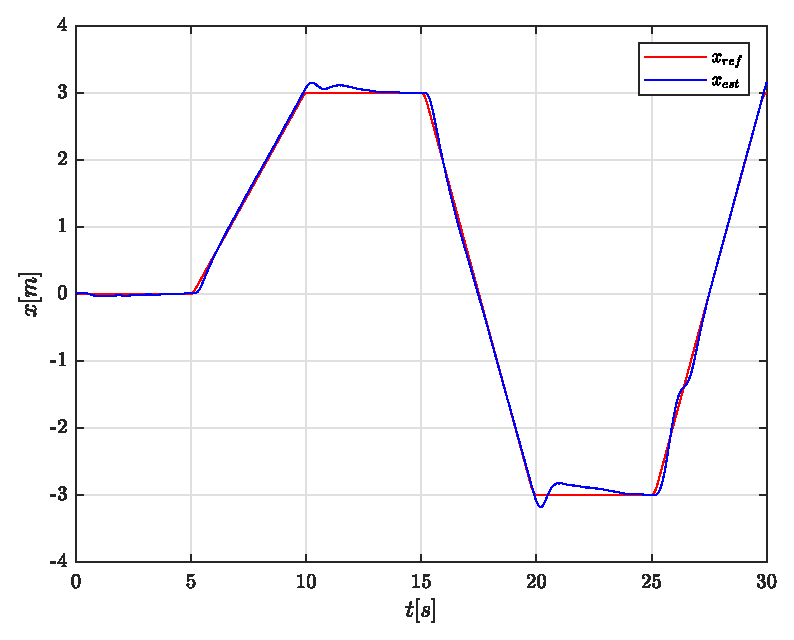
\includegraphics[width=1\textwidth]{Simulazioni/Figure/SMC/BUTTERFLY/PositionControlXPos}
		\caption{Controllo posizione lungo x}
	\end{subfigure}
	\hfill
	\begin{subfigure}{0.45\textwidth}
		\centering
		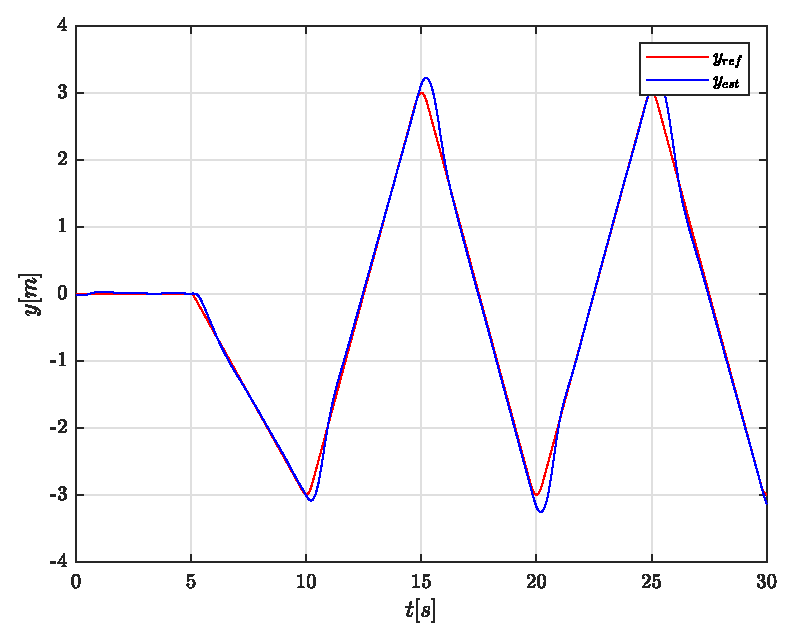
\includegraphics[width=1\textwidth]{Simulazioni/Figure/SMC/BUTTERFLY/PositionControlYPos}
		\caption{Controllo posizione lungo y}
	\end{subfigure}
	\\
	\begin{subfigure}{0.45\textwidth}
		\centering
		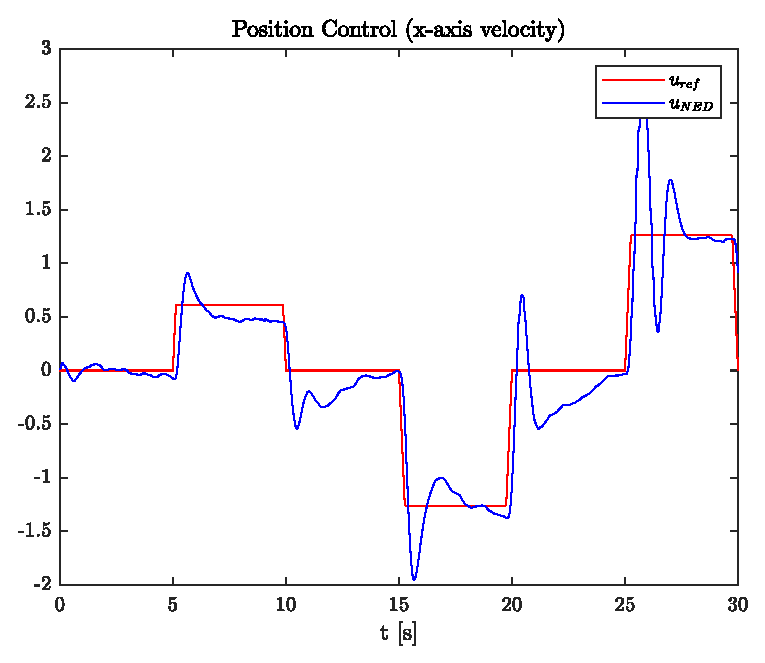
\includegraphics[width=1\textwidth]{Simulazioni/Figure/SMC/BUTTERFLY/PositionControlXVel}
		\caption{Controllo velocità lungo x}
	\end{subfigure}
	\hfill
	\begin{subfigure}{0.45\textwidth}
		\centering
		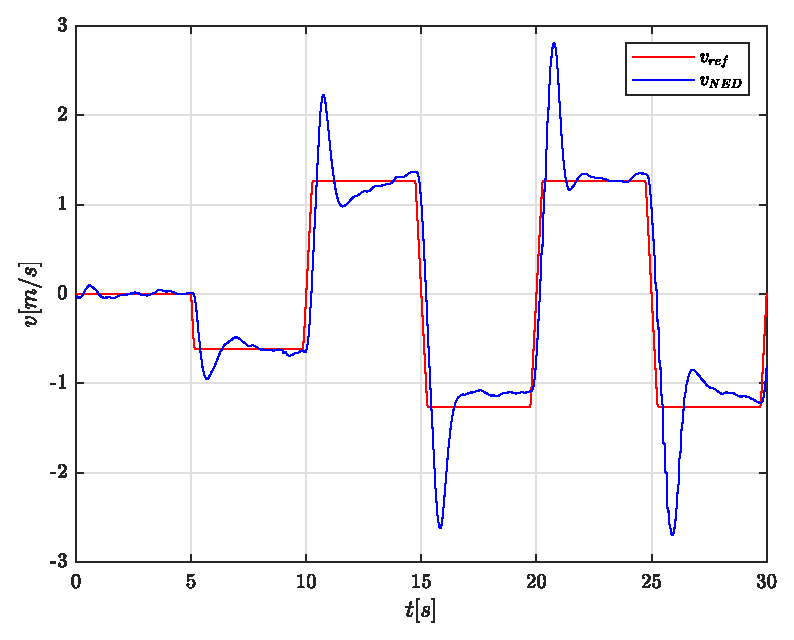
\includegraphics[width=1\textwidth]{Simulazioni/Figure/SMC/BUTTERFLY/PositionControlYVel}
		\caption{Controllo velocità lungo y}
	\end{subfigure}
	\caption{Risposta in posizione con controllore interno SMC al comando BUTTERFLY}
\end{figure}

\begin{figure}
	\centering
	\begin{subfigure}{0.45\textwidth}
		\centering
		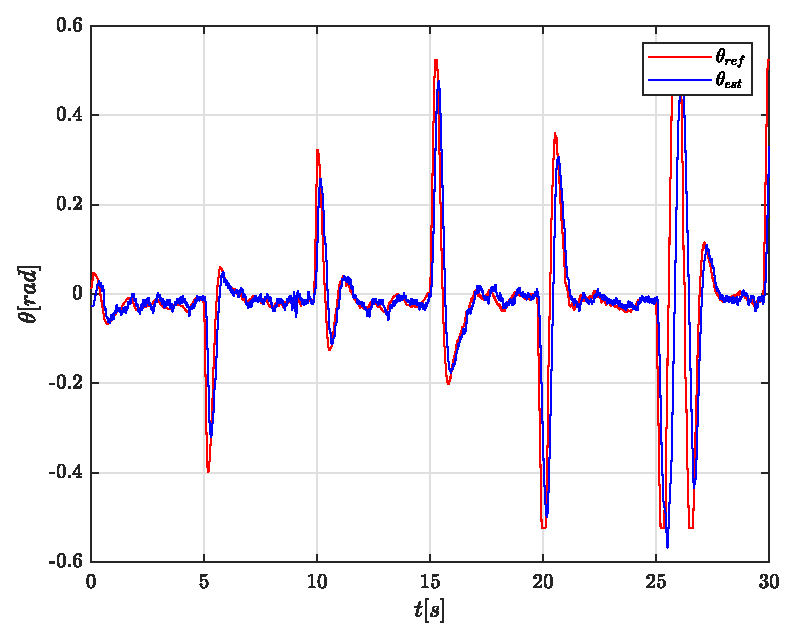
\includegraphics[width=1\textwidth]{Simulazioni/Figure/SMC/BUTTERFLY/AttitudeControlPitch}
		\caption{Controllo beccheggio}
	\end{subfigure}
	\hfill
	\begin{subfigure}{0.45\textwidth}
		\centering
		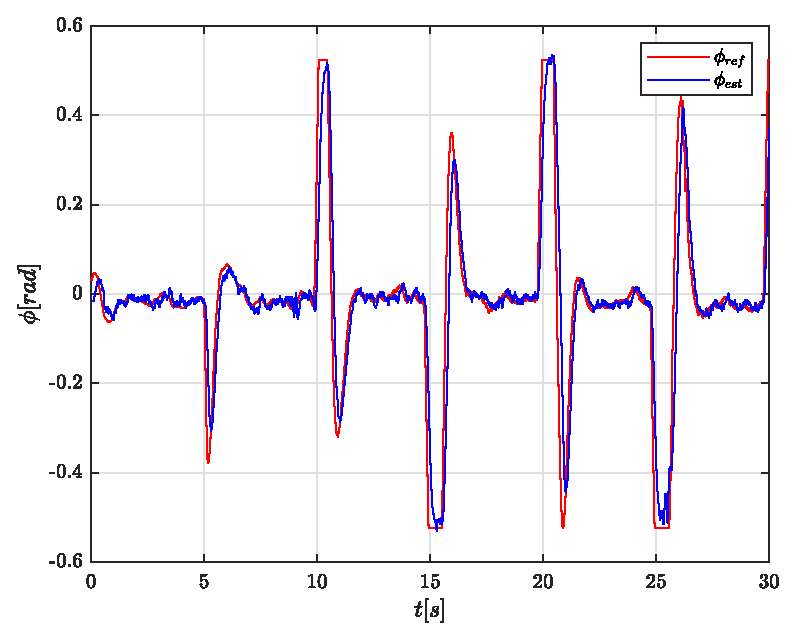
\includegraphics[width=1\textwidth]{Simulazioni/Figure/SMC/BUTTERFLY/AttitudeControlRoll}
		\caption{Controllo rollio}
	\end{subfigure}
	\hfill
	\begin{subfigure}{0.45\textwidth}
		\centering
		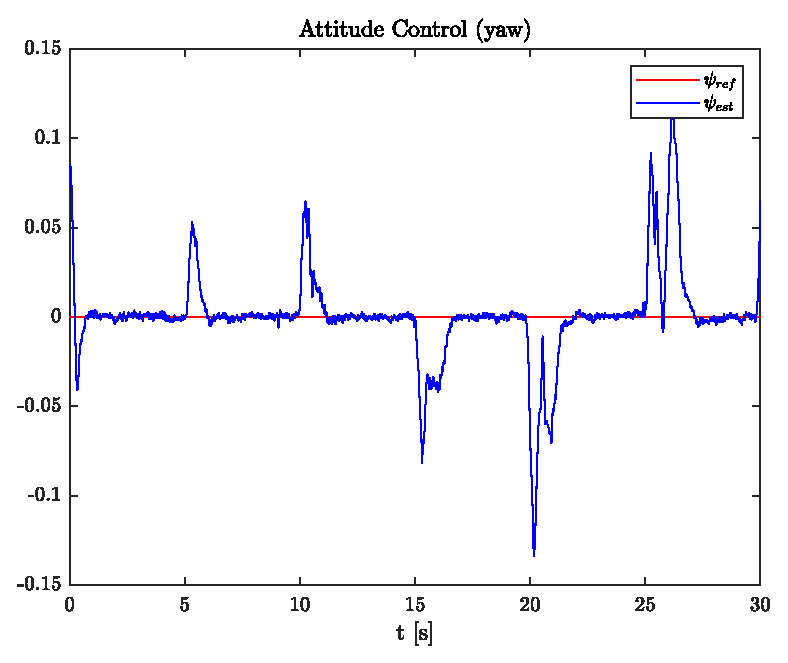
\includegraphics[width=1\textwidth]{Simulazioni/Figure/SMC/BUTTERFLY/AttitudeControlYaw}
		\caption{Controllo imbardata}
	\end{subfigure}
	\caption{Risposta dell' assetto con controllore interno SMC al comando BUTTERFLY}
\end{figure}

\begin{figure}
	\centering
	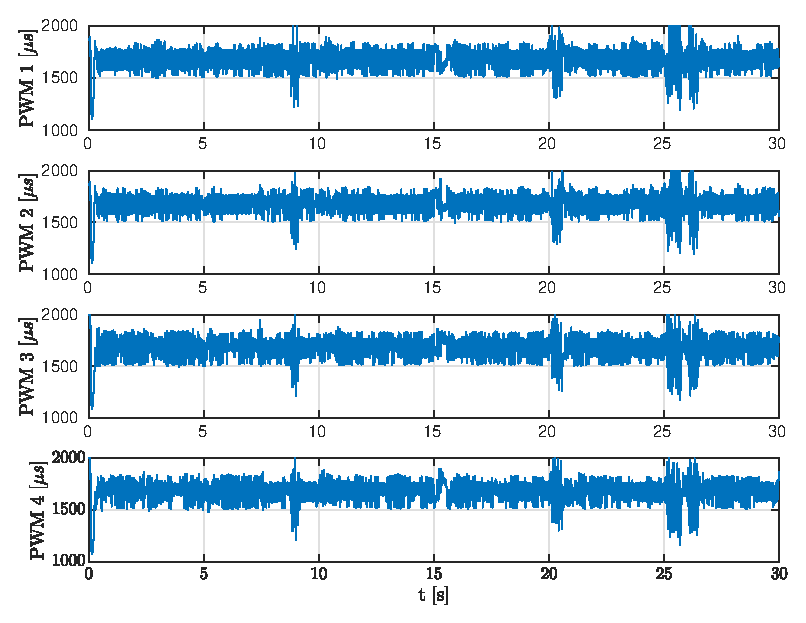
\includegraphics[width=0.5\textwidth]{Simulazioni/Figure/SMC/BUTTERFLY/PWM}
	\caption{Segnali PWM del controllore SMC al segnale BUTTERFLY}
\end{figure}
\begin{figure}
	\centering
	\includegraphics[width=1\textwidth]{Simulazioni/Figure/SMC/BUTTERFLY/Trajectory}
	\caption{Traiettoria percorsa con controllore SMC al segnale BUTTERFLY}
\end{figure}

\clearpage
\subsubsection{SNAKE}
\begin{figure}
	\centering
	\begin{subfigure}{0.45\textwidth}
		\centering
		\includegraphics[width=1\textwidth]{Simulazioni/Figure/SMC/SNAKE/PositionControlXPos}
		\caption{Controllo posizione lungo x}
	\end{subfigure}
	\hfill
	\begin{subfigure}{0.45\textwidth}
		\centering
		\includegraphics[width=1\textwidth]{Simulazioni/Figure/SMC/SNAKE/PositionControlYPos}
		\caption{Controllo posizione lungo y}
	\end{subfigure}
	\\
	\begin{subfigure}{0.45\textwidth}
		\centering
		\includegraphics[width=1\textwidth]{Simulazioni/Figure/SMC/SNAKE/PositionControlXVel}
		\caption{Controllo velocità lungo x}
	\end{subfigure}
	\hfill
	\begin{subfigure}{0.45\textwidth}
		\centering
		\includegraphics[width=1\textwidth]{Simulazioni/Figure/SMC/SNAKE/PositionControlYVel}
		\caption{Controllo velocità lungo y}
	\end{subfigure}
	\caption{Risposta in posizione con controllore interno SMC al comando SNAKE}
\end{figure}

\begin{figure}
	\centering
	\begin{subfigure}{0.45\textwidth}
		\centering
		\includegraphics[width=1\textwidth]{Simulazioni/Figure/SMC/SNAKE/AttitudeControlPitch}
		\caption{Controllo beccheggio}
	\end{subfigure}
	\hfill
	\begin{subfigure}{0.45\textwidth}
		\centering
		\includegraphics[width=1\textwidth]{Simulazioni/Figure/SMC/SNAKE/AttitudeControlRoll}
		\caption{Controllo rollio}
	\end{subfigure}
	\hfill
	\begin{subfigure}{0.45\textwidth}
		\centering
		\includegraphics[width=1\textwidth]{Simulazioni/Figure/SMC/SNAKE/AttitudeControlYaw}
		\caption{Controllo imbardata}
	\end{subfigure}
	\caption{Risposta dell' assetto con controllore interno SMC al comando SNAKE}
\end{figure}


\begin{figure}
	\centering
	\includegraphics[width=0.5\textwidth]{Simulazioni/Figure/SMC/SNAKE/PWM}
	\caption{Segnali PWM del controllore SMC al segnale SNAKE}
\end{figure}
\begin{figure}
	\centering
	\includegraphics[width=1\textwidth]{Simulazioni/Figure/SMC/SNAKE/Trajectory}
	\caption{Traiettoria percorsa con controllore SMC al segnale SNAKE}
\end{figure}


\clearpage
\subsection{Confronto}
\todo[inline]{Descrizione della precisione maggiore del SMC rispetto al PID a discapito del consumo maggiore}